\documentclass[11pt]{article}

% ENCODAGE CARACTERES
\usepackage[utf8]{inputenc}
\usepackage[T1]{fontenc}
\usepackage[frenchb]{babel}

% MISE EN FORME
\usepackage[left=3cm,right=3cm,top=3cm,bottom=3cm]{geometry}
\usepackage[colorlinks=true,urlcolor=blue]{hyperref}
\usepackage{xcolor}
\usepackage{enumitem}
\usepackage{pifont}
\usepackage{graphicx}
\usepackage{listings}
\usepackage{placeins}

\hypersetup{linkcolor=blue}

\frenchbsetup{StandardLists=true}
\setitemize[0]{font=\color{black},label=\ding{227},itemsep=0pt}

\title{Projet Kameleon - Dossier de synthèse}
\author{Ny Sitraka FIDIMIHAJAMANANA \and Alexis BONNIN}
\date{Avril 2017}

\begin{document}

\maketitle
\begin{abstract}
    Vous trouverez dans ce document un dossier de synthèse du projet Kameleon. Ce dernier a consisté au développement d'une application client/serveur mettant en oeuvre un protocole de communication en réseau.
\end{abstract}
\tableofcontents
\newpage

\section{Introduction}
    
    \paragraph{}
    Le projet Kameleon s'inscrit dans le module "Réseaux" du master ALMA et a consisté en la réalisation d'un Chat en mode client/serveur. Cette application gère des échanges de messages entre des machines distantes via un serveur qui administre les connexions des utilisateurs. L'application est divisée en deux parties : une partie "serveur" déployée sur un seul poste et une partie "cliente" utilisée simultanément sur plusieurs postes. L'objectif du projet était de mieux comprendre le mécanisme de socket du modèle TCP/IP. Vous trouverez dans ce rapport une présentation des sockets, une description du protocole implémenté, le détail de la réalisation ainsi que des jeux d'essais du programme.

    \paragraph{}
    Le projet est disponible sur github à l'adresse : \url{https://github.com/Asteip/SocketProject.git}. Pour installer le projet, il suffit d'exécuter la commande \textit{make} à la racine du répertoire. Le programme peut ensuite être exécuté avec les commandes suivantes :
    
    \begin{enumerate}
        \item Lancer le serveur :
        \begin{lstlisting}[language=bash,captionpos=b]
        $ ./server
        \end{lstlisting}
        
        \item Lancer un client :
        \begin{lstlisting}[language=bash,captionpos=b]
        # adresse-serveur : adresse IP du serveur distant
        # pseudo : pseudo du client, ce dernier ne doit 
        # pas contenir d'espace.
        $ ./client <adresse-serveur> <pseudo (sans espace)>
        \end{lstlisting}
    \end{enumerate}
    
    Il se peut que le client ne fonctionne pas correctement lors du lancement de celui-ci et que des caractères étranges apparaissent à l'écran. Pour corriger ce problème, il suffit de relancer le client.    

\section{Présentation des sockets}

    \subsection{Généralités}
    Le socket est l'élément principal de ce projet. Il permet la connexion entre deux programmes et facilite ainsi l'envoi/recéption des données entre les deux processus. En effet, les deux processus doivent adopter un protocole de communication afin d'assurer l'échange de données. Deux modes de communication sont proposés :
    \begin{itemize}
        \item \textbf{le mode connecté} : comparable à une communication téléphonique utilisant le protocole TCP (détails ci-après). Dans ce mode de communication, une connexion durable est établie entre les deux processus, de telle façon que l’adresse de destination n’est pas nécessaire à chaque envoi de données.
        \item \textbf{le mode déconnecté} (analogue à une communication par courrier), utilisant le protocole UDP. Ce mode nécessite l’adresse de destination à chaque envoi, et aucun accusé de réception n’est donné. Ni l'unicité ni la séquentialité des transferts n'est garantie. Ce mode n'est pas fiable, il peut y avoir des pertes.
    \end{itemize}
    
    
    \subsection{Le protocole TCP}
     TCP, \textit{Transmission Control Protocol}, est un protocole de communication fiable en mode connecté. Dans le modèle Internet, aussi appelé modèle TCP/IP, TCP est situé au-dessus de IP. Dans le modèle OSI, il correspond à la couche transport, intermédiaire de la couche réseau et de la couche session. Une session TCP fonctionne en trois phases : 
    \begin{itemize}
        \item ouverture de la connexion
        \item transfert des données
        \item fermeture de la connexion
    \end{itemize}
    
    Dans ce projet, ces trois phases sont effectués par les fonctions de socket ci-dessous :
    \begin{itemize}
        \item \textbf{connect(...) / accept(...)} \\
        La fonction \textit{connect} établie une connexion avec un serveur. C'est une fonction bloquante, c'est-à-dire qu'elle ne rend la main que lorsque la connexion est effectivement établie ou s'il y a une erreur de connexion.\\
        La fonction \textit{accept} est exécutée du côté du serveur, elle prend la première demande en attente. Elle crée ensuite un nouveau socket et retourne le déscripteur de ce socket. La connexion est alors établie entre le client et le serveur.
        \item \textbf{read(...) / write(...)}\\
        Ces fonctions sont nécessaires pour le transfert des données. Elles sont semblables aux fonctions d'écriture et lecture de fichiers.
        
        \item \textbf{close(...)}\\
        Cette fonction permet de fermer un socket dont on donne le descripteur en paramètre. Dans le mode connecté, le système essaie d'envoyer les données restantes avant de fermer le socket.
    \end{itemize}
        
    Le protocole TCP assure la bonne transmission des données (sans perte) mais aussi la séquentialité (l'ordre) de celles-ci. C'est pourquoi nous avons opté pour le mode connecté dans ce projet.
\section{Cahier des charges}
\label{sec:cahier-des-charges}

    Cette partie présente les objectifs que nous nous sommes fixés au début du projet. Elle contient les fonctionnalités que nous avons pu implémenter et celles-que nous souhaitions mettre en place mais qui n'ont pas été implémentées. Vous trouverez donc les différentes spécifications de l'application, c'est-à-dire les fonctionnalités du chat.

    \subsection{Fonctionnalités implémentées}
    
        \subsubsection{Envois de messages}
            L'envoi de message est la fonctionnalité la plus importante de l'application. Un message envoyé par un client doit passer par le serveur pour être traité, puis envoyé au(x) destinataire(s).
            
            On distingue deux types de messages :            
            \begin{itemize}
                \item Les messages "basiques" : messages textuels
                \item Les messages "évolués" : envoi de fichiers (.png, .txt, etc.)
            \end{itemize}
            
            On détaillera dans cette partie l'envoi de messages basiques, l'envoi de messages évolués n'étant pas implémentée pour cette application, celui-ci sera expliqué dans la section~\ref{subsec:fct-non-implemente}.
            
            Tout d'abord, lorsqu'un client se connecte au serveur, il lui est possible d'envoyer des messages textuels. Par défaut, ce dernier est alors diffusé à tous les autres utilisateurs connectés. Il est possible de spécifier des commandes spéciales dans le messages (ces commandes seront détaillées dans la section~\ref{sec:detail-realisation}). Un client peut également choisir, via une de ces commandes, d'envoyer son message à un destinataire unique (fonction message privé). Ce dernier doit être connecté au serveur.          
            
        \subsubsection{Gestion de la connexion au serveur}
            La connexion au serveur est obligatoire pour communiquer avec les autres clients. Cette fonctionnalité est donc essentielle et doit permettre à n'importe quel client connecté au réseau et connaissant l'adresse IP du serveur de se connecter.
            
            Tout d'abord, pour se connecter au serveur, le client doit fournir l'adresse IP de celui-ci ainsi qu'un pseudonyme unique. Si un client du même nom est déjà connecté au serveur alors l'utilisateur devra modifier son nom afin de se connecter. Les informations de chaque client sont stockées sur le serveur et ne sont pas toutes visibles des autres utilisateurs. Parmi ces informations, on retrouve le numéro de socket utilisé par le client ainsi que son pseudonyme.        
        
        \subsubsection{Gestion des erreurs}
            La gestion des erreurs concerne en grande partie le serveur. En effet, si le message envoyé par un client ne peut être transmis, alors le serveur doit pouvoir gérer ce cas. 
            
            Pour le chat Kameleon, la gestion d'erreur suivante a été mise en place :    
            \begin{itemize}
                \item Si le serveur ne reçoit pas un message, l'utilisateur qui a envoyé le message reçoit une notification.
                \item Tant qu'un message n'a pas été reçu par tous les utilisateurs, le serveur conserve le message dans une file d'attente. Si un utilisateur du salon n'a pas reçu le message (ie : erreur de transmission serveur -> client), alors le serveur renvoie à cet utilisateur, uniquement, le message. Dès que le message est reçu par tous les utilisateurs, le serveur supprime le message de sa file d'attente. Si le message ne peut pas être transmis à tous les utilisateurs au bout d'un certain temps alors le serveur supprime le message. 
                \item Dans le cas d'un message privé, tant qu'un message n'a pas été reçu par son destinataire, le serveur conserve le message dans une file d'attente. Si le destinataire n'a pas reçu le message, alors le message est renvoyé. Dès que le message est reçu, le serveur supprime le message de sa file d'attente. Si le message ne peut pas être transmis au bout d'un certain temps, alors le serveur supprime le message et envoi une notification à l'émetteur.
            \end{itemize}
        
    \subsection{Fonctionnalités non implentées}
    \label{subsec:fct-non-implemente}
        
        \subsubsection{Gestion de salons}
            La gestion de salon était une de nos premières idées quand à la réalisation du chat. En effet, nous souhaitions nous rapprocher le plus possible du mode de fonctionnement d'un chat tel que \href{https://www.skype.com/fr/}{Skype}. Nous n'avons malheureusement pas pu implémenter cette fonctionnalité.
            
            Un salon doit respecter les règles suivantes :
            \begin{itemize}
                \item Un salon est créé par un client, ce dernier devient alors l'administrateur de ce salon.
                \item Chaque client peut ouvrir jusqu'à 3 salons.
                \item L'administrateur d'un salon défini le nombre de personne maximum pouvant se connecter au salon.
                \item Chaque client peut se connecter à un salon existant s'il reste de la place.
                \item Un message envoyé par un client sur un salon est diffusé à tous les autres utilisateurs connectés à ce salon.
                \item Lors de la connexion d'un client au serveur, ce dernier lui renvoi la liste des salons ouverts.
            \end{itemize}
        
        \subsubsection{Envoi de messages "évolués"}
            L'envoi de message dit "évolué" n'a pas été implémenté pour cette application. Ce type de message concerne l'envoi de petit fichiers tel que des images.
            
            L'envoi de fichier doit respecter les règles suivantes : 
            \begin{itemize}
                \item La taille totale du message ne doit pas dépasser 10Mo.
                \item Le fichier doit pouvoir être lu et traité par le serveur.
            \end{itemize}
\section{Détails de la réalisation}
\label{sec:detail-realisation}
    
    Cette partie détaille les fonctionnalités qui ont été réalisées pour cette application ainsi que les possibles évolution de ces dernières. Elle présente également les difficultés rencontrées lors du développement.

    \subsection{Fonctionnalités réalisées}
        \paragraph{}
        Tout d'abord, sur l'application cliente, nous avons géré l'envoi et la réception de messages avec deux thread. Le premier thread (\textit{envoi()}) est exécuté à chaque fois que l'utilisateur saisie un message et l'envoi. La fonction utilisée pour ce thread prend en paramètre le numéro du socket sur lequel le client est connecté ainsi que le message à envoyer. Le deuxième thread est lancé dès que le client se connecte au serveur et reste s'exécute tant que la connexion est active. La fonction utilisée pour ce thread requiert le numéro de socket utilisé sur le serveur afin de pouvoir rester à l'écoute de ce dernier. Ce thread se termine dans les cas suivants : si le client ferme le programme (Ctrl + c), si le serveur est inaccessible (fermeture du programme, coupure réseau, etc.) ou si le client se déconnecte du serveur. Le programme principal se termine une fois que tous les thread sont terminés.
        
        L'application cliente possède une interface graphique développée à l'aide de la librairie ncurses. Elle divise l'écran en deux parties : une fenêtre (en haut) permettant d'afficher les messages reçus du serveur et une fenêtre (en bas) permettant de saisir les messages à envoyer. Le nom de l'utilisateur est affiché en haut du terminal.
        
        \paragraph{}
        Pour ce qui est de l'application serveur, celle-ci permet la gestion d'un nombre illimité de client. En effet, deux tableaux dynamiques (vecteurs) permettent de stocker pour chaque client connecté, d'une part les socket et d'autre part les pseudonymes. Ces tableaux sont remplis en parallèles, c'est-à-dire que le numéro de socket et le pseudo du client X sont sauvegardés à la même case dans les deux tableaux. Ainsi, lorsqu'un client se connecte ou se déconnecte ces deux tableaux sont mis à jour.
        
        Le serveur reste à l'écoute d'éventuels clients, chaque fois qu'un client se connecte, un numéro de socket lui est attribué et un nouveau thread est exécuté et reste actif le temps de la connexion du client. Nous utilisons donc le mode connecté des sockets, qui utilise le protocole TCP. Lorsqu'un client se déconnecte, le socket qu'il utilisait peut être réattribué à un nouveau client. Il reste cependant inutilisable pendant quelques instants après la déconnexion.
        
        Le serveur actuel ne gère qu'un seul salon. Tout client se connectant au serveur sera automatiquement ajouté à ce salon. Ainsi, lorsqu'un utilisateur envoi un message, ce dernier est diffusé à tous les autres client connectés au serveur. De plus, lorsqu'un client se connecte ou se déconnecte, une notification est envoyée à chaque client.
        
        Pour terminer, nous avons mis en place une gestion d'erreur côté serveur. Lorsqu'un message ne peut pas être transmis à un client (problème de réseau), le message, le socket du client destinataire ainsi qu'un compteur sont stockés dans trois tableaux différents à la même case. Un thread, démarré dès le lancement du serveur, est chargé de vider cette liste en permanence en renvoyant le message au destinataire en question. Le compteur permet de gérer le timeout : celui-ci est initialisé à une valeur X (3 la plupart du temps) et est décrémenté à chaque tour de boucle. Lorsqu'il tombe à zéro, le message non envoyé est supprimé de la liste
        
        \paragraph{}
        Concernant l'application Kameleon en général, nous avons décidé d'imposer les règles suivantes : 
        \begin{itemize}
            \item La taille totale d'un message ne doit pas dépasser 255 caractères (226 caractères pour le message texte, 20 caractères pour le pseudonyme et 10 caractères de marge).
            \item La taille d'un pseudo est limitée à 20 caractères.
            \item Chaque pseudonyme est unique.
        \end{itemize}
        
        \paragraph{}
        Des commandes sont disponibles dans l'application. Chaque commandes doit être précédée d'un "/" et suivie des éventuelles options. Les commandes suivantes sont disponibles pour chaque client :
        \begin{itemize}
            \item \textbf{/q} : cette commande permet de quitter l'application, le client est alors déconnecté du serveur et son application se ferme.
            
            \item \textbf{/w} : cette commande permet d'envoyer un message privé. Elle doit être suivie du pseudonyme du destinataire. Si ce dernier n'est pas connecté alors le message d'erreur suivant est renvoyé à l'émetteur : "Le client n'existe pas".
            
            \item \textbf{/l} : cette commande permet de lister les pseudonymes des utilisateurs actuellement connectés au serveur.
            
            \item \textbf{/n} : cette commande permet à un client de changer son pseudonyme. Elle doit être suivie d'un nouveau nom respectant les règles établies précédemment (taille limitée à 20 et nom unique). Si le nom ne respecte pas une des règles, alors un message d'erreur est renvoyé au client.
            
            \item \textbf{/h} : cette commande permet d'afficher l'aide, c'est-à-dire les différentes commandes existantes.
        \end{itemize}
    
    \subsection{Évolutions de l'application et problèmes persistants}
        \paragraph{}
        Des problèmes subsistent dans la dernière version de l'application. Nous avons en effet rencontré certaines difficultés concernant la gestion des chaînes de caractères en C et plus particulièrement sur l'affichage avec ncurses. Ainsi, l'envoi d'une chaîne de caractère trop longue pour être affichée sur une seule ligne entraînera des bugs graphiques. De plus, il arrive que lors du lancement de l'application cliente, des caractères apparaissent à l'écran. Ceci est dû à la libraire ncurses qui n'est pas thread safe et qui peut ainsi occasionner des bugs graphiques lorsqu'elle s'initialise mal. 
        
        Concernant la commande "/l", nous avons réussit à contourner le problème d'affichage sur une ligne en modifiant la forme de la réponse. Ainsi, le serveur n'enverra pas la liste complète des utilisateurs connectés en un seul message mais enverra un message pour chaque utilisateur connecté contenant un seul pseudonyme suivi d'un délais, afin d'éviter les problèmes de buffer dans l'affichage.
        
        \paragraph{}
        Concernant les évolutions possibles de l'application, l'ajout d'un système de salon géré par les clients pourrait être envisagé. Il pourrait également être possible d'envoyer des fichiers, qui seraient alors transmis différemment des messages textuels.
        
\section{Jeux d'essais}

    Cette partie présente les principales fonctionnalités de l'application au travers de captures d'écrans.
    
    \paragraph{}
    L'image~\ref{fig:lancement_serveur} ci-dessous montre l'écran affiché lors du démarrage du serveur. On peut voir le numéro de port à utiliser : 5000.
    \begin{figure}[!htpb]
        \centering
        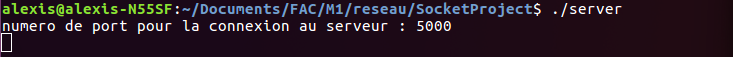
\includegraphics[width=10cm]{captures/lancement_serveur.png}
        \caption{\textit{Démarrage du serveur}}
        \label{fig:lancement_serveur}
    \end{figure}
    
    \FloatBarrier
    
    \paragraph{}
    L'image~\ref{fig:lancement_client} ci-dessous montre l'écran de démarrage d'un client se connectant au serveur. On peut apercevoir le message "test s'est connecté", ce qui montre bien que la connexion est réussie.
    \begin{figure}[!htpb]
        \centering
        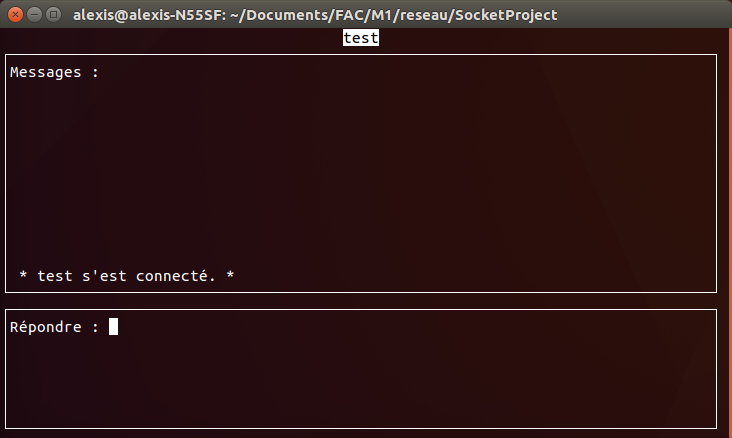
\includegraphics[width=10cm]{captures/lancement_client.png}
        \caption{\textit{Démarrage du client}}
        \label{fig:lancement_client}
    \end{figure}
    
    \FloatBarrier
    
    \paragraph{}
    L'image~\ref{fig:erreur_connexion} ci-dessous montre le message d'erreur affiché lorsque les paramètres de connexion chez le client sont mal renseignés.
    \begin{figure}[!htpb]
        \centering
        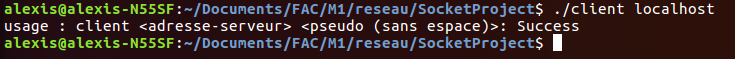
\includegraphics[width=10cm]{captures/erreur_connexion.png}
        \caption{\textit{Erreur de connexion}}
        \label{fig:erreur_connexion}
    \end{figure}
    
    \FloatBarrier
    
    \paragraph{}
    L'image~\ref{fig:connexion_serveur} ci-dessous montre que le client "test" s'est connecté sur le serveur et possède le numéro de socket "4".
    \begin{figure}[!htpb]
        \centering
        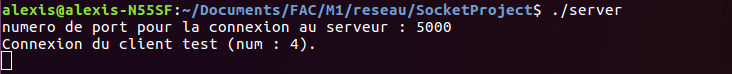
\includegraphics[width=10cm]{captures/connexion_serveur.png}
        \caption{\textit{Connexion sur le serveur}}
        \label{fig:connexion_serveur}
    \end{figure}
    
    \FloatBarrier
    
    \paragraph{}
    L'image~\ref{fig:cmd_help} ci-dessous montre le résultat de la commande "help".
    \begin{figure}[!htpb]
        \centering
        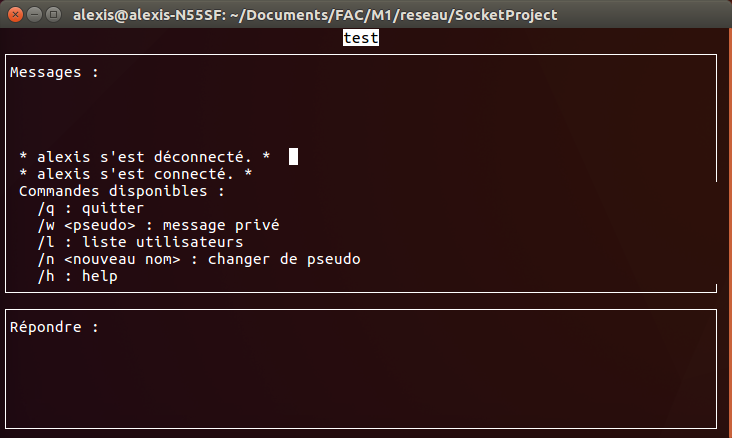
\includegraphics[width=10cm]{captures/cmd_help.png}
        \caption{\textit{Commande /h}}
        \label{fig:cmd_help}
    \end{figure}
    
    \FloatBarrier
    
    \paragraph{}
    L'image~\ref{fig:cmd_liste_utilisateurs} ci-dessous montre le résultat de la commande "liste utilisateurs". Ici trois utilisateurs sont connectés au serveur.
    \begin{figure}[!htpb]
        \centering
        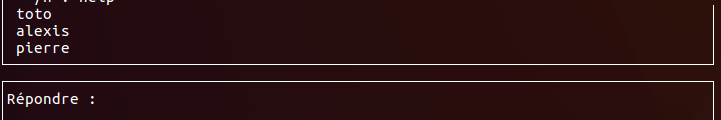
\includegraphics[width=10cm]{captures/cmd_liste_utilisateurs.png}
        \caption{\textit{Commande /l}}
        \label{fig:cmd_liste_utilisateurs}
    \end{figure}
    
    \FloatBarrier
    
    \paragraph{}
    L'image~\ref{fig:cmd_mp} ci-dessous montre le résultat de la commande "message privé" suivi du pseudo du destinataire : "alexis".
    \begin{figure}[!htpb]
        \centering
        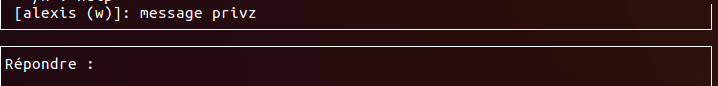
\includegraphics[width=10cm]{captures/cmd_mp.png}
        \caption{\textit{Commande /w}}
        \label{fig:cmd_mp}
    \end{figure}
    
    \FloatBarrier
    
    \paragraph{}
    L'image~\ref{fig:cmd_mp_erreur} ci-dessous montre le résultat de la commande "message privé" avec une erreur : "Le client n'existe pas".
    \begin{figure}[!htpb]
        \centering
        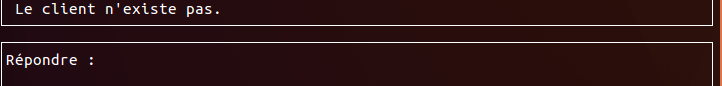
\includegraphics[width=10cm]{captures/cmd_mp_erreur.png}
        \caption{\textit{Commande /w avec erreur}}
        \label{fig:cmd_mp_erreur}
    \end{figure}
    
    \FloatBarrier
    
    \paragraph{}
    L'image~\ref{fig:cmd_renommage} ci-dessous montre le résultat de la commande "changer de pseudo" suivi du pseudo "toto".
    \begin{figure}[!htpb]
        \centering
        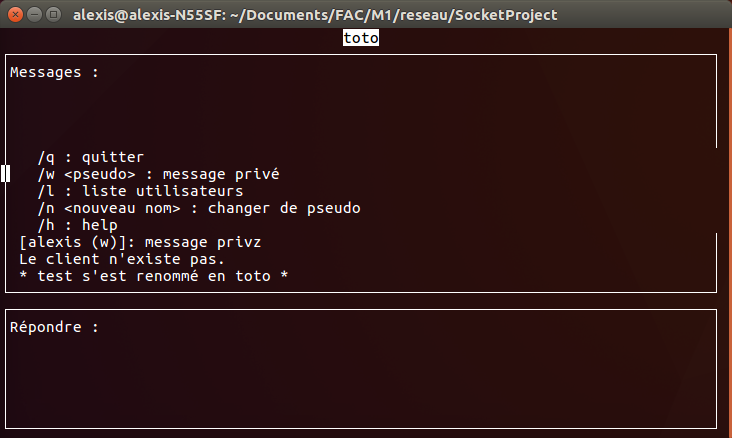
\includegraphics[width=10cm]{captures/cmd_renommage.png}
        \caption{\textit{Commande /n}}
        \label{fig:cmd_renommage}
    \end{figure}
    
    \FloatBarrier
    
    \paragraph{}
    L'image~\ref{fig:deconnexion_client} ci-dessous montre la déconnexion d'un autre client (ici la déconnexion de toto).
    \begin{figure}[!htpb]
        \centering
        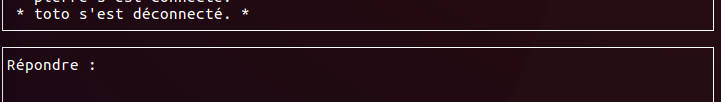
\includegraphics[width=10cm]{captures/deconnexion_client.png}
        \caption{\textit{Déconnexion d'un client}}
        \label{fig:deconnexion_client}
    \end{figure}
    
    \FloatBarrier
    
    \paragraph{}
    L'image~\ref{fig:deconnexion_serveur} ci-dessous montre la déconnexion de toto sur le serveur. Le numéro de socket "4" est désormais disponible.
    \begin{figure}[!htpb]
        \centering
        
\includegraphics[width=10cm]{captures/deconnexion_serveur.png}
        \caption{\textit{Déconnexion d'un client (vue serveur)}}
        \label{fig:deconnexion_serveur}
    \end{figure}

\FloatBarrier

\section{Conclusion}
    
    Ce projet nous a permis de comprendre le fonctionnement des sockets. Nous avons pu développer une application fonctionnelle avec une interface terminale assez correcte: Kameleon. Cette dernière a pu illustrer les différents enjeux d'utilisation des sockets en mode connecté. On a pu revoir ainsi les principes de fonctionnement du protocole TCP. Les difficultés rencontrées sont principalement liées à l'interface: l'affichage des caractères avec une présentation correcte.      
    
\end{document}
